%% analyse.tex
%% $Id: analyse.tex 28 2007-01-18 16:31:32Z bless $

\chapter{Analyse}
\label{ch:Analyse}
%% ==============================

Nach der Klarstellung der grundlegenden Begrifflichkeiten im vorhergehenden Kapitel
sollen nun die Anforderungen und Limitationen einer Studie festgestellt werden, die den
Zusammenhang zwischen der Nutzung von Social Media, Instant Messaging und der Geselligkeit
von Nutzern untersuchen soll. 
Dazu werden auch bereits existierende Lösungsansätze betrachtet. 

%% ==============================
\section{Anforderungen}
%% ==============================
\label{ch:Analyse:sec:Anforderungen}

%Anforderungen und Randbedingungen\index{Randbedingungen} \ldots

Für die Untersuchung des Zusammenhanges werden zwei Datenpunkte benötigt.
Auf der einen Seite ein wie auch immer gearteter Wert für die Geselligkeit der Probandin. 
Dem gegenüberstehend wird ein Datensatz der Informationen über das Nutzungsverhalten ebenjener Probandin enthält benötigt.
\par

\subsection{Geselligkeit}

Um die Geselligkeit der Studienteilnehmerinnen festzustellen wird, entsprechend des Big Five Persönlichkeitsmodells, ein von Psychologen entwickelter Selbstbewertungsfragebogen eingesetzt.
Der NEO-Personality Inventory-Revised Fragebogen ist ein in wissenschaftlichen Studien häufig

jadajdajajdajdjajd.

\subsection{Nutzungsdaten}

Von besonderer Relevanz für das Sammeln der Nutzungsdaten ist es festzulegen welche Daten zur Verfügung stehen, welche relevant sind und welche potenziell trotzdem nicht gesammelt werden sollten.
Für diese Arbeit werden keine Nutzerdaten von physische Sensoren in Betracht gezogen, sondern nur die Interaktion mit dem Smartphone als Kommunikationsgerät.
Zu diesem Zweck interagiert die Applikation mit Schnittstellen des Android Betriebssystems.
Dies vermeidet das potenzielle Problem von unterschiedlicher Hardware und sorgt dafür, dass die Nutzungsdaten von allen Testprobanden vergleichbar bleiben.
Zudem vermeidet dies übermäßige Mehrbelastung der Akkuleistung der Smartphones, auf denen die Applikation installiert wird.
Allgemein ist es wünschenswert die Belastung der Resourcen auf den Zielgeräten so gering wie möglich zu halten.
\par

Eine der stärksten Limitation für die Daten, die die Applikation sammeln kann, kommt von der Natur der zu betrachtenden Daten.
Zum einen begrenzt das Android Betriebssystem selbst die Informationen zu denen eine Applikation, selbst eine die vom Nutzer mit potenziell jeder Berechtigung ausgestattet wurde, Zugang hat.
Dies geschieht aus Datenschutz gründen, da manche Applikationen im Play Store mehr Berechtigungen einfordern als sie für ihr Funktionieren benötigen würden.
Zum anderen sind die Kommunikationsapplikationen, die die Testprobandin nutzt von unabhängigen Drittentwicklern entworfen worden.
Einige Wenige von diesen stellen in ganz speziellen Fällen, zum Beispiel Twitter\cite{twitterapi}, zwar eine API zur Verfügung, die meisten hüten ihre Daten aber.
Folglich können nur Daten gesammelt werden, die entweder frei zugänglich sind, oder solche, zu denen die Nutzerin Applikationen Zugriff erlauben kann.
Beispiele hierfür sind zum Beispiel die Call logs in denen Android, für alle Apps mit der \textbf{android.permission.READ\_CALL_LOG} Berechtigung, die vergangenen Anrufe abspeichert.
\par

In diesem Kontext ist das Android API Ziellevel der Applikation von großer Bedeutung.
Wie bei Smartphone Betriebssystemen üblich wird das Android Betriebssystem konstant weiterentwickelt und neue Versionen davon werden ausgeliefert.
Potenzielle Änderungen an Systemschnittstellen werden dabei durch die verschiedenen API Levels dokumentiert, auf die sich installierte Applikationen berufen können.
Die aktuellste Version von Android ist Android 6.0, oder auch Android Marshmallow.
Diese wird representiert durch das API Level 23.
Da nicht alle Geräte aber die steigenden Anforderungen der neueren Android Versionen erfüllen, 
und manche Nutzer neu herauskommende Updates selbst dann nicht installieren, wenn ihr Gerät sie unterstützt, 
sei es auf Grund von Faulheit, Unwissenheit oder Bequemlichkeit, sind auf vielen Smartphones ältere Android Versionen vertreten.
Eine Übersicht über die Verteilung der Android Versionen sieht man in \ref{fig:androidplatformdistr}.
Mit 36.1\% ist Android 5, beziehungsweise Android Lollipop die am weitesten verbreitetste Version,
gefolgt von Android 4.4 (Kitkat) mit 34.3\% und Android 4.0-4.3 (Jellybean) mit 22.3\%\cite{androiddistr}.
Für die Entwicklung der Applikation wird Android API level 21, entspricht Android 5.0, als Ziellevel bestimmt, da es einige relevante Schnittstellen hinzufügt die bei niedrigeren Leveln noch nicht existieren, aber auch eine breit genuge Userbasis hat, um ausreichend viele Probanden zu finden.


\begin{figure}[h]
    \centering
    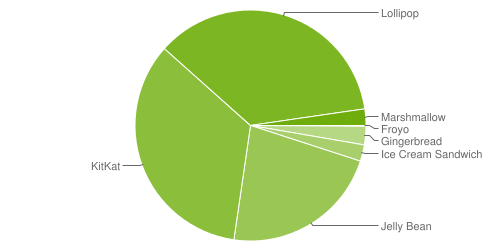
\includegraphics{images/chart.png}
    \caption{Android Platform Distribution\cite{androiddistr}}
    \label{fig:androidplatformdistr}
\end{figure}

Auch die Empfindungen potenzieller Testprobandinnen müssen in Betracht gezogen werden:
Während die Anzahl an Anrufen in den vergangenen 14 Tagen von vielen als Unkritisch betrachtet werden würde, so gibt es sicher eine Menge Menschen, 
die eine Liste von Telefongesprächen inklusive Zeitpunkt und Rufnummer des Partners als zu tiefen Eingriff wahrnehmen würden.
Ziel muss es hier sein bezüglich der Geselligkeit aussagekräftige Datenpunkte zu wählen, 
die aber dennoch nicht das grundlegende Bedürfnis nach Privatsphäre der Probandinnen verletzt.


\subsection{Datenschutz}

Die Daten mit denen im Rahmen dieser Studie gearbeitet werden sind sehr sensibler Natur.
Dementsprechend muss sicher gestellt werden, dass sowohl die Anonymität der einzelnen Probandinnen gewahrt bleibt,
als auch dass die Daten nicht den Rahmen der Studie verlassen.
Dazu werden die erhobenen Daten pseudonymisiert, das heißt zur Indenfikation der Zugehörigkeit von Fragebogen und erhobenen Daten wird nicht der Name der Versuchsteilnehmerin genutzt sondern ein frei gewähltes Pseudonym.
Außerdem werden keinerlei persönlichkeitsbezogene Daten im Klartext gespeichert.
Weder Telefonnummern, noch Absender oder Nachrichten Inhalte werden in Klartext geloggt.
Stattdessen werden die relevanten Features der Daten in anderer Form abgespeichert:
Unter anderem Anzahl verschiedener Telefonnummern, durch Hashen unkenntlich gemachte Nachrichtenabsender und Ersetzen der Nachrichtentexte durch die Anzahl der Zeichen in der Nachricht.
Dennoch wird, wie bei allen Studien dieser Art, die am TECO durchgeführt werden,
eine unterschriebene Einwilligungserklärung seitens der Probandin benötigt.
In dieser wird das Einverständnis der Probandin bezüglich der Aufzeichnung, Speicherung und Verarbeitung zugesichert.
\ignore{siehe Anhang, adde anhang?}
\par



%% ==============================
\section{Existierende Lösungsansätze}
%% ==============================
\label{ch:Analyse:sec:RelatedWork}

Hier kommt eine ausführliche Diskussion
von "`Related Work"'.

Bla fasel\ldots

%% ==============================
\section{Weiterer Abschnitt}
%% ==============================
\label{ch:Analyse:sec:Abschnitt}


  \ignore{Bla fasel\ldots hat auch schon \cite{TB20} gesagt und
\cite{TB98,JSAC96,qosr} sollte man mal gelesen haben.
Abbildung~\ref{fig:test} auf S.~\pageref{fig:test} sollte man
sich mal anschauen.}

Blindtext Blindtext Blindtext Blindtext Blindtext Blindtext Blindtext
Blindtext Blindtext Blindtext Blindtext Blindtext Blindtext Blindtext
Blindtext Blindtext Blindtext Blindtext Blindtext Blindtext Blindtext
Blindtext Blindtext Blindtext Blindtext Blindtext Blindtext Blindtext
Blindtext Blindtext Blindtext Blindtext Blindtext Blindtext Blindtext
Blindtext Blindtext Blindtext Blindtext Blindtext Blindtext Blindtext
Blindtext Blindtext Blindtext Blindtext Blindtext Blindtext Blindtext
Blindtext Blindtext Blindtext Blindtext Blindtext Blindtext Blindtext
Blindtext Blindtext Blindtext Blindtext Blindtext Blindtext Blindtext

Blindtext Blindtext Blindtext Blindtext Blindtext Blindtext Blindtext
Blindtext Blindtext Blindtext Blindtext Blindtext Blindtext Blindtext
Blindtext Blindtext Blindtext Blindtext Blindtext Blindtext Blindtext
Blindtext Blindtext Blindtext Blindtext Blindtext Blindtext Blindtext
Blindtext Blindtext Blindtext Blindtext Blindtext Blindtext Blindtext
Blindtext Blindtext Blindtext Blindtext Blindtext Blindtext Blindtext
Blindtext Blindtext Blindtext Blindtext Blindtext Blindtext Blindtext
Blindtext Blindtext Blindtext Blindtext Blindtext Blindtext Blindtext
Blindtext Blindtext Blindtext Blindtext Blindtext Blindtext Blindtext
Blindtext Blindtext Blindtext Blindtext Blindtext Blindtext Blindtext
Blindtext Blindtext Blindtext Blindtext Blindtext Blindtext Blindtext
Blindtext Blindtext Blindtext Blindtext Blindtext Blindtext Blindtext
Blindtext Blindtext Blindtext Blindtext Blindtext Blindtext Blindtext

Blindtext Blindtext Blindtext Blindtext Blindtext Blindtext Blindtext
Blindtext Blindtext Blindtext Blindtext Blindtext Blindtext Blindtext
Blindtext Blindtext Blindtext Blindtext Blindtext Blindtext Blindtext
Blindtext Blindtext Blindtext Blindtext Blindtext Blindtext Blindtext
Blindtext Blindtext Blindtext Blindtext Blindtext Blindtext Blindtext
Blindtext Blindtext Blindtext Blindtext Blindtext Blindtext Blindtext
Blindtext Blindtext Blindtext Blindtext Blindtext Blindtext Blindtext
Blindtext Blindtext Blindtext Blindtext Blindtext Blindtext Blindtext
Blindtext Blindtext Blindtext Blindtext Blindtext Blindtext Blindtext
Blindtext Blindtext Blindtext Blindtext Blindtext Blindtext Blindtext

Blindtext Blindtext Blindtext Blindtext Blindtext Blindtext Blindtext
Blindtext Blindtext Blindtext Blindtext Blindtext Blindtext Blindtext
Blindtext Blindtext Blindtext Blindtext Blindtext Blindtext Blindtext
Blindtext Blindtext Blindtext Blindtext Blindtext Blindtext Blindtext
Blindtext Blindtext Blindtext Blindtext Blindtext Blindtext Blindtext
Blindtext Blindtext Blindtext Blindtext Blindtext Blindtext Blindtext
Blindtext Blindtext Blindtext Blindtext Blindtext Blindtext Blindtext
Blindtext Blindtext Blindtext\index{Blindtext} Blindtext Blindtext Blindtext Blindtext

\begin{figure}[!htbp]
  \centering
  \fbox{\parbox{0.8\textwidth}{
  Abbildungen sollten möglichst als EPS (Encapsulated Postscript) 
  bzw. PDF eingebunden werden.
  Zur Erzeugung sauberer EPS-Dateien empfiehlt sich das Tool \texttt{ps2eps}
  zur Nachbearbeitung von Postscript-Dateien. Mit \texttt{epstopdf} kann
  dann eine PDF-Datei zum Einbinden erzeugt werden.}}
  \caption{Testabbildung}
  \label{fig:test}
\end{figure}

Blindtext Blindtext Blindtext Blindtext Blindtext Blindtext Blindtext
Blindtext Blindtext Blindtext Blindtext Blindtext Blindtext Blindtext
Blindtext Blindtext Blindtext Blindtext Blindtext Blindtext Blindtext
Blindtext Blindtext Blindtext Blindtext Blindtext Blindtext Blindtext
Blindtext Blindtext Blindtext Blindtext Blindtext Blindtext Blindtext
Blindtext Blindtext Blindtext Blindtext Blindtext Blindtext Blindtext
Blindtext Blindtext Blindtext Blindtext Blindtext Blindtext Blindtext

Blindtext Blindtext Blindtext Blindtext Blindtext Blindtext Blindtext
Blindtext Blindtext Blindtext Blindtext Blindtext Blindtext Blindtext
Blindtext Blindtext Blindtext Blindtext Blindtext Blindtext Blindtext

Blindtext Blindtext Blindtext Blindtext Blindtext Blindtext Blindtext
Blindtext Blindtext Blindtext Blindtext Blindtext Blindtext Blindtext
Blindtext Blindtext Blindtext Blindtext Blindtext Blindtext Blindtext
Blindtext Blindtext Blindtext Blindtext Blindtext Blindtext Blindtext
Blindtext Blindtext Blindtext Blindtext Blindtext Blindtext Blindtext
Blindtext Blindtext Blindtext Blindtext Blindtext Blindtext Blindtext

Blindtext Blindtext Blindtext Blindtext Blindtext Blindtext Blindtext
Blindtext Blindtext Blindtext Blindtext Blindtext Blindtext Blindtext
Blindtext Blindtext Blindtext Blindtext Blindtext Blindtext Blindtext
Blindtext Blindtext Blindtext Blindtext Blindtext Blindtext Blindtext
Blindtext Blindtext Blindtext Blindtext Blindtext Blindtext Blindtext
Blindtext Blindtext Blindtext Blindtext Blindtext Blindtext Blindtext
Blindtext Blindtext Blindtext Blindtext Blindtext Blindtext Blindtext
Blindtext Blindtext Blindtext Blindtext Blindtext Blindtext Blindtext
Blindtext Blindtext Blindtext Blindtext Blindtext Blindtext Blindtext
Blindtext Blindtext Blindtext Blindtext Blindtext Blindtext Blindtext
Blindtext Blindtext Blindtext Blindtext Blindtext Blindtext Blindtext
Blindtext Blindtext Blindtext Blindtext Blindtext Blindtext Blindtext
Blindtext Blindtext Blindtext Blindtext Blindtext Blindtext Blindtext
Blindtext Blindtext Blindtext Blindtext Blindtext Blindtext Blindtext

Blindtext Blindtext Blindtext Blindtext Blindtext Blindtext Blindtext
Blindtext Blindtext Blindtext Blindtext Blindtext Blindtext Blindtext
Blindtext Blindtext Blindtext Blindtext Blindtext Blindtext Blindtext
Blindtext Blindtext Blindtext Blindtext Blindtext Blindtext Blindtext
Blindtext Blindtext Blindtext Blindtext Blindtext Blindtext Blindtext
Blindtext Blindtext Blindtext Blindtext Blindtext Blindtext Blindtext
Blindtext Blindtext Blindtext Blindtext Blindtext Blindtext Blindtext
Blindtext Blindtext Blindtext Blindtext Blindtext Blindtext Blindtext
Blindtext Blindtext Blindtext Blindtext Blindtext Blindtext Blindtext
Blindtext Blindtext Blindtext Blindtext Blindtext Blindtext Blindtext
Blindtext Blindtext Blindtext Blindtext Blindtext Blindtext Blindtext
%% ==============================
\section{Zusammenfassung}
%% ==============================
\label{ch:Analyse:sec:zusammenfassung}

Am Ende sollten ggf. die wichtigsten Ergebnisse nochmal in \emph{einem}
kurzen Absatz zusammengefasst werden.

%%% Local Variables: 
%%% mode: latex
%%% TeX-master: "diplarb"
%%% End: 
